\chapter{Communication entre deux terminaux}
\section{Quels sont les éléments constitutifs d'un système de communication ?}
Considérons deux terminaux qui veulent communiquer. Chaque terminal contient, en plus de
l'unité émettrice/ réceptrice des données, une unité de contrôle de la communication. Le
signal généré par le terminal peut ne pas être adapté au support de communication. On rajoute
alors un équipement d'adaptation du signal au support (par ex. un modem pour la connexion de
l'ordinateur au réseau téléphonique). Ces équipements d'adaptation forment les extrémités du
Circuit de Données.

\begin{figure}[H]
	\centering
	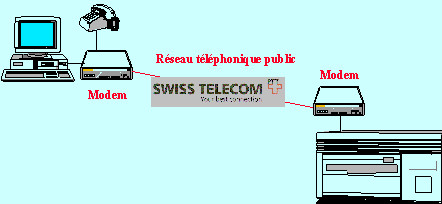
\includegraphics[width=8cm]{partie2/transmodem.jpg}
\end{figure}

Le terminal est appelé ETTD\footnote{Equipement Terminal de Traitement de Données} ou
DTE\footnote{Data
Terminal Equipment}. L'équipement d'adaptation est appelé ETCD (Equipement de Terminaison du
Circuit de Données) ou DCE\footnote{Data Circuit terminating Equipment ou Data Communication
Equipment}.
\begin{figure}[H]
	\centering
	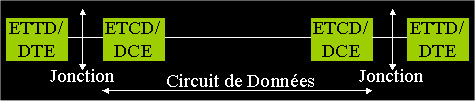
\includegraphics[width=8cm]{partie2/ettdetcd.jpg}
\end{figure}
L'interface ETTD/ETCD (DTE/DCE) a été normalisée ainsi que la communication entre ETCD. La
normalisation permet de concevoir des ETCD indépendemment des ETTD et de faire communiquer des
ETCD entre eux même s'ils ne proviennent pas du même constructeur.


\section{Qu'appelle-t-on transmission parallèle et transmission série ?}
u début, la communication a été développée pour mettre en relation les hommes et leur
permettre de dialoguer. Lorsque les caractères ont été codifiés, on a pensé à émettre
caractère par caractère. Si l'usage du morse en utilisant une ligne pour la propagation du
signal électrique transmettait les éléments significatifs d'un caractère l'un à la suite de
l'autre (en série), l'apparition des équipements avec un clavier favorisera la transmission
des éléments significatifs en parallèle (propagation de plusieurs signaux électriques sur
plusieurs lignes en parallèle).

En informatique, la transmission parallèle consiste à envoyer les différents bits d'un
caractère en parallèle, tandis que dans la transmission série, les bits sont envoyés l'un
après l'autre (bit de poids faible en tête par convention).

L'avantage principal de la transmission parallèle est d'envoyer plus de bits. En réalité, cet
avantage est atténué par des inconvénients majeurs, principalement sur des distances
importantes et à des débits élevés:

\begin{itemize}
	\item coût plus important du à l'utilisation de plus de fils pour la propagation;
	\item encombrement plus important;
	\item synchronisation entre signaux délicate du au fait que la vitesse de propagation d'un signal
\end{itemize}
est dépendant de facteurs inhérents au support et au signal; le déphasage introduit (aussi
minime soit il) augmente avec la distance. En plus, en augmentant le débit, la durée d'un bit
diminue et le déphasage induit un décalage de bits. Ainsi, les bits représentant un caractère
n'arrivent pas en même temps.

C'est pourquoi, la transmission parallèle est réservée pour des distances assez courtes et on
utilise la transmission série pour les réseaux.

Comme la transmission est effectuée en parallèle au sein du calculateur, une conversion
parallèle/série (et vice versa) est nécessaire pour émettre/recevoir en série. Cette opération
est réalisée au moyen de registre à décalage.


\section{Quelles sont les différences entre une transmission asynchrone et une transmission synchrone ?}
Comme nous l'avons vu précédemment, la transmission s'est effectuée à ses débuts caractère par
caractère. En effet, l'équipement terminal utilisé permet chaque fois que l'utilisateur appuit
sur une touche d'émettre un caractère. La durée séparant deux caractères est aléatoire
dépendant de la frappe de l'utilisateur. La transmission se fait caractère par caractère d'une
manière asynchrone.

La question qui se pose alors est la détection du début de transmission d'un caractère sans
introduire d'autres fils véhiculant d'autres signaux. De plus, les horloges d'émission et de
réception doivent être en phase. Or la durée entre caractères est complètement aléatoire et
par conséquent n'est pas obligatoirement multiple de la fréquence de l'horloge.

La solution proposée est la suivante:
On utilise deux états pour le signal (E1 et E2). La ligne au repos correspond à l'émission
d'un signal dans l'état E1. Lorsqu'un caractère va être émis, l'équipement émetteur envoie un
signal à l'état E2 durant la durée d'un bit (START of transmission). La transition E1-E2
permet à l'horloge récepteur de se caler pour la réception d'un caractère. Après la fin de
l'émission d'un caractère (l'équipement émetteur et récepteur connaissent la longueur d'un
caractère), l'émetteur remet la ligne à l'état repos (E1), c'est le signal d'arrêt de
transmission (STOP of transmission) qui dure un bit, un bit et demi ou deux bits.Cet arrêt de
transmission permet de détecter un nouveau caractère. La durée du STOP prévu au début d'un bit
a été augmentée pour prendre en compte le temps de traitement de certains équipements avant la
réception d'un nouveau caractère. Bien sûr, si cela n'est pas suffisant et l'émetteur est
``trop rapide'', alors des caractères de bourrage peuvent être envoyés ou le flux de
l'émetteur doit être contrôlé. Mais, il faut signaler que la transmssion asynchrone est prévu
pour des transmissions à bas débit.

Ainsi, la transmission asynchrone est une transmission où les unités de données sont envoyées
d'une manière asynchrone. Comme l'unité de donnée, au début, était le caractère, la
transmission asynchrone est une transmission caractère par caractère. On l'appelle aussi
transmission START/STOP.
\begin{figure}[H]
	\centering
	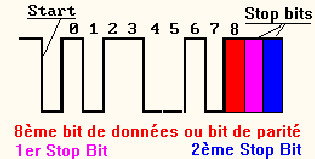
\includegraphics[width=8cm]{partie2/asynchrone.jpg}
\end{figure}
Lorsque l'entité émettrice fournit les caractères à un niveau plus élevé. Les caractères se
suivent sur le support sans temps d'attente entre deux caractères si ce n'est le STOP-START.
Or la présence de ces deux états devient inutile et gaspille l'utilisation du support. La
solution est de constituer un bloc de caractères et d'effectuer une transmission par blocs. La
transmission devient synchrone caractère. Une horloge caractère est nécessaire à l'arrivée
pour retrouver les différents caractères. La structuration en blocs va permettre la
réalisation de protocoles plus sophistiqués. Toutefois, la transmission n'étant pas continue,
il faut déterminer le début d'un bloc et la fin d'un bloc (dans le cas où la taille est
variable). Le préambule du bloc sert aussi à la synchronisation des horloges Emission et
Réception. Nous pouvons distinguer deux types de transmission synchrones caractères: la
transmission asynchrone bloc lorsque la durée séparant deux blocs est quelconque et la
transmission synchrone bloc lorsque la durée séparant deux blocs n'est pas quelconque mais un
multiple de la cadence de l'horloge. Ceci peut être obtenue en envoyant entre deux blocs une
suite de caractères de synchronisation.

\section{Comment résout-on le problème de synchronisation des horloges Emission et Réception ?}
La désynchronisation des horloges d'émission et de réception est du à deux causes:

\begin{itemize}
	\item les horloges, bien qu'ayant la même fréquence nominale, peuvent avoir une légère dérive;
	\item la vitesse de propagation du signal dépend de la fréquence du signal. Cette variation bien
que légère est problématique sur de longues distances et à des débits élevés.
\end{itemize}

Pour résoudre ces problèmes, il faut caler l'horloge de réception sur l'horloge d'émission. Ce
verouillage est effectué au début de la transmission de l'unité de donnée et il faut éviter
qu'une dérive significative ait lieu avant la fin de sa transmission. Nous remarquons donc
qu'une dérive importante ne peut avoir lieu dans la transmission asynchrone. En effet, si on
décale d'un bit tous les huit bits (par ex.), il y a un problème sérieux au niveau des
horloges !!!

Le problème se situe donc au niveau de la transmission synchrone. Deux solutions peuvent être
utilisées:

\begin{itemize}
	\item transmettre le signal d'horloge sur un fil à part; ceci est concevable sur des courtes
distances mais sur de longues distances, un déphasage entre le signal de données et le signal
d'horloge peut se produire du à la variation de vitesse de propagation;
	\item recaler l'horloge de réception en se basant sur le signal de données; en effet les
transitions (fronts) dans un signal sont des instants significatifs permettant aux horloges de
se mettre en phase; plus un signal est riche en transitions plus la synchronisation est
assurée;
\end{itemize}

Pour avoir suffisamment d'instants significatifs deux techniques sont utilisés:

\begin{itemize}
	\item introduire régulièrement des caractères de synchronisation (riches en transitions 01 et/ou
10 se traduisant par des transitions d'états);
\item effectuer un codage information/signal riche en transitions (ex. codage biphase - chaque bit
est codé par deux états et donc avec un transition);
\end{itemize}


\section{Qu'appelle-t-on transmission simplex et transmission duplex ?}
Considérons deux équipements A et B. Si les données sont émis dans un seul sens de A vers B,
la transmission est unidirectionnelle ou simplex.

Si les données peuvent être émis dans les deux sens, la transmission est bidirectionnelle ou
duplex. On distingue le Half Duplex (ou alternat) le cas où les données sont transmis dans un
sens à un instant donné et change ensuite de sens; et le Full Duplex (ou simultané) le cas où
les données peuvent être transmis dans les deux sens en même temps.


\section{Combien de fils sont nécessaires pour la transmission ?}
Nous nous intéressons uniquement à la transmission série et aux fils nécessaires pour
véhiculer les données et au signal de terre pour des raisons électriques. D'autres fils
peuvent être nécessaires dans certains cas pour véhiculer les signaux d'horloge ou pour
véhiculer les signaux de contrôle de la communication.

Dans le cas d'une liaison simplex, deux fils suffisent (données + terre).

Dans le cas d'une liaison half-duplex, deux fils suffisent. Ce sont les équipements
d'extrémité qui se retourneront.

Dans le cas d'une liaison full-duplex, quatre fils peuvent être nécessaires (2 paires). Il est
possible dans certains cas d'utiliser une terre commune.

D'autres configurations sont possibles:

\begin{itemize}
	\item half-duplex avec quatre fils: cette configuration permet l'exploitation en half duplex la
liaison utilisant des équipements sans retournement (parcequ'ils ne peuvent pas se retourner
(présence d'amplis) ou pour gangner du temps);
\item full-duplex avec deux fils: un canal fréquentiel est utilisé dans un sens et un autre canal
dans un autre sens. c'est la technique du multiplexage fréquentiel;
\end{itemize}


\section{Quelle est la différence entre débit binaire et rapidité de modulation ?}
Le débit binaire mesure la quantité d'informations binaires émises par unité de temps (Bits
par seconde (bps)).

En terme de quantité, on distingue les bas débits (bps), les moyens débits (Kbps), les hauts
débits (Mbps) et les très hauts débits (Gbps).

Le débit est relatif à l'entité émettrice/réceptrice. Ainsi, le débit ligne désigne la
quantité d'information émise sur le support (information utile et de contrôle). Le débit utile
(ou effectif) caractérise la quantité d'information utile envoyée. Le débit de l'application
prend en compte différents facteurs dont les temps d'attente inhérents au protocole et au
réseaux traversés. C'est ainsi qu'un débit de transfert de fichiers avec un équipement
emetteur à 10Mbps, peut atteindre 50bps. De la même façon que le débit utile peut dépasser
dans certains cas le débit support en utilisant des techniques de compression. Souvent qu'on
on parle de débit sans préciser autre chose, il s'agit de débit ligne.

Nous avons vu que l'information est représentée sous forme d'un signal pour la transmission.
La rapidité de modulation caractérise le nombre de changements d'états (ou nombre d'états) par
unité de temps. Prenoms comme unité le nombre d'états par seconde.

Nous appelons valence le nombre d'états utilisés pour représenter l'information. Ainsi, si on
utilise deux états (par ex. +5 volts pour le bit 1 et 0v pour le bit 0) la valence est de 2 et
les signal est bivalent. Mais un état de signal peut représenter, non pas un bit, mais
plusieurs bits. C'est la multivalence (Valence >2). Ainsi, en codant les dibits (ensemble de 2
bits), la valence est de 4 ($2^2$). Pour un débit donné, la multivalence permet de générer un
signal plus adapté au support. Ainsi, sur le réseau téléphonique, la multivalence a permis
d'augmenter les débits. Mais, l'augmentation du nombre d'états augmente la difficulté de
discrimination sachant que les défauts du support introduisent des distorsions des états
utilisés.

Trouvons maintenant la relation entre débit binaire et rapidité de modulation. Nous appelons n
le nombre de bits représentés par un état, V la valence d'un signal, D le débit et R la
rapidité de modulation. Nous avons $D=n\times R$. Or $V=2^n$ et $n=\log_2(V)$. D'où
$D=R\times\log_2(V)$. Nous voyons
que le débit binaire et la rapidité de modulation ne sont identiques que lorsque la valence
est 2.

La rapidité de modulation est exprimée en Bauds (du nom de l'ingénieur Baudot). Elle
caractérise le signal transmis.








